The weak lensing analysis process can be conceptually split into two parts; 1) converting images to catalogs of galaxy shapes and 2) extracting scientific results from shape catalogs. In this section we present a sample image to catalog pipeline. 

\begin{figure}
    \begin{small}
        \begin{center}
            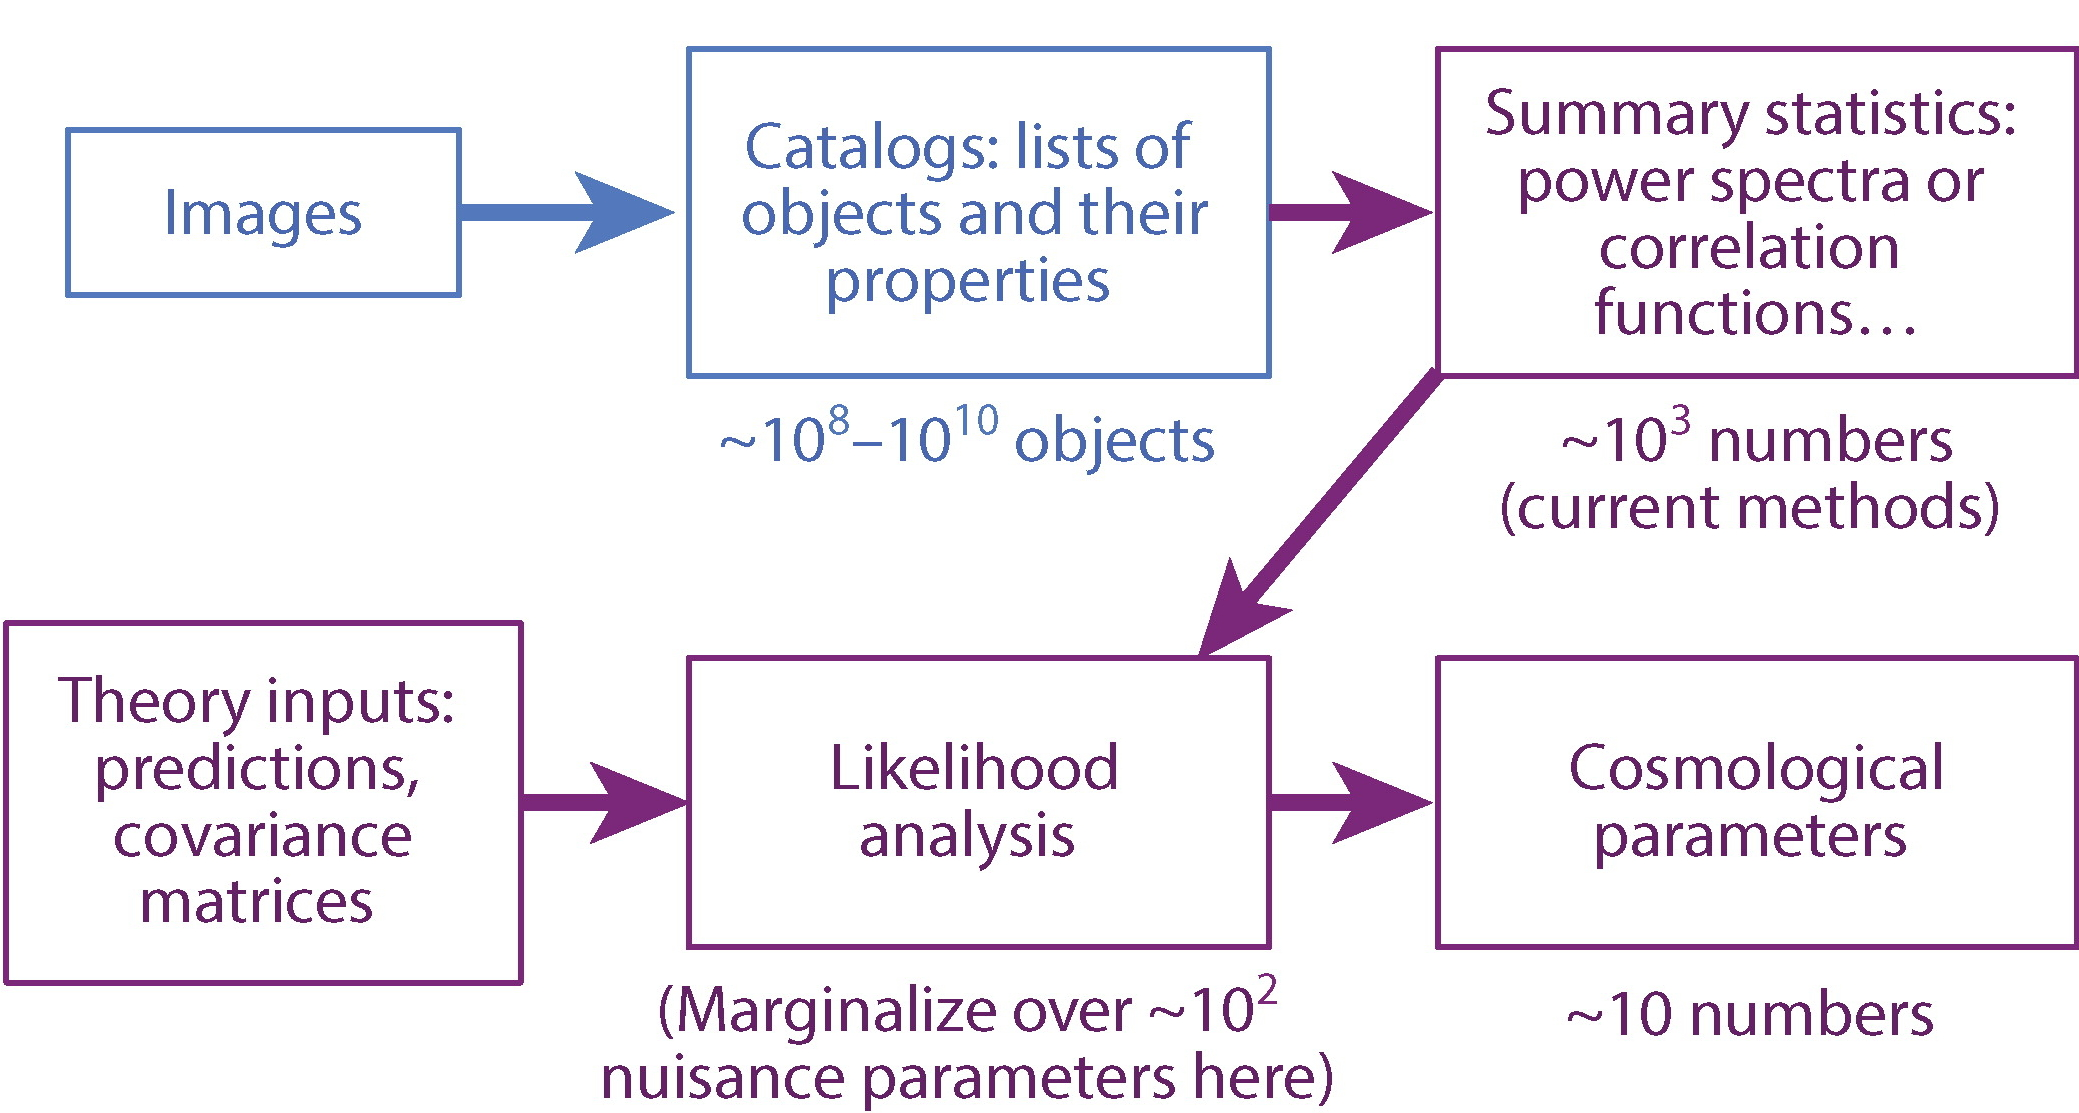
\includegraphics[width=0.95\textwidth]{figs/pipe.jpg}
        \end{center}
        \caption{A generic outline of weak lensing pipeline analysis as presented in \cite{rachel_2018}}
        \label{fig:pipe}
    \end{small}
\end{figure}


\subsubsection{Object Detection and Deblending}

The first step in weak lensing analysis is to detect the objects that will be analyzed. The objects used for cosmological applications of weak lensing are galaxies. Galaxies are detected using diffraction limited optical systems with a large field of view in order to enable accurate measurements of the galaxy shapes. 

\subsubsection{Point Spread Function}

The point spread function (PSF) describes the response of an imaging system to a point source or point object. In practice the surface brightness profile of an object in an image is not the $f_{obs}$ from \autoref{eq:linearizedbright} but is convoloved with some unknown function $PSF(\vec{x})$. Therefore, in order to detect weak lensing signal we must understand and reconstruct our PSF in order to deconvolve it from the image. Deconvolving the PSF is the most important and most difficult step of any weak lensing analysis \cite{Hoekstra:2013gua,rachel_2018}. The PSF has a width which leads to rounder images and typically is anisotropic, which leads to a preferred orientation. The bias is grouped into two kinds: a multiplicative bias $m$ that scales the shear, and an additive bias $c$ that reflects preferred orientations that are introduced. The observed shear and true shear are thus related by

\begin{equation}
    \gamma_{obs} = (1+m) \gamma + c
     \label{eq:shearobs}
\end{equation}




\subsubsection{Shape Extraction}
talk about moments etc



